\chapter{UCNA Experiment}
\label{ch:UCNA_Experiment}
%%%%%%%%%%%%%%%%%%%%%%%%%%%%%%%%%%%%%%%%%%%%%%%%%%%%%%%%%%%%%%%%%%%%%%%%%%%%%%%
%%%%%%%%%%%%%%%%%%%%%%%%%%%%%%%%%%%%%%%%%%%%%%%%%%%%%%%%%%%%%%%%%%%%%%%%%%%%%%%
%%%%%%%%%%%%%%%%%%%%%%%%%%%%%%%%%%%%%%%%%%%%%%%%%%%%%%%%%%%%%%%%%%%%%%%%%%%%%%%

The UCNA Experiment is a mature experiment, having taken data from
2007-2013, that aims to precisely determine $A_{0}$, the neutron
$\beta$-decay asymmetry parameter. Here a description of the experimental
apparatus is given, as well as previous measurements
of $A_{0}$ from other experiments for comparison.

The description which follows applies to data taken from Fall 2011 through
Spring 2013. The analysis is split into two separate data sets, 2011-2012
and 2012-2013, due to minor changes in the decay trap geometries. Although
small, any changes in the geometry prompt new simulations, and so a separate
analysis is carried out. From now on, any part of the experiment or analysis
which is different for the two data sets will be indicated.

\section{Overview}
\label{sec:Overview}

Ultracold neutrons are produced in a solid deuterium source which is fed
neutrons via a spallation source at the end of an $800$ MeV
proton beam. These UCN are then guided towards a material trap where they
decay. During travel, the UCN pass through a series of polarizing magnets
which allows the experimenter to control the spin state of the neutrons in
the trap during any run. Utilizing a $~1$~T magnetic field along the central
axis of the decay volume, decay electrons spiral towards detectors at either end of
the spectrometer where their energy can be reconstructed. From knowledge about
the initial direction and the energy of the neutron, one can construct an
energy dependent asymmetry and determine a value for $A_{0}$.

%%%%%%%%%%%%%%%%%%%%%%%%%%%%%%%%%%%%%%%%%%%%%%%%%%%%%%%%%%%%%%%%%%%%%%%%%%%%%%%
%%%%%%%%%%%%%%%%%%%%%%%%%%%%%%%%%%%%%%%%%%%%%%%%%%%%%%%%%%%%%%%%%%%%%%%%%%%%%%%
\section{Ultracold Neutron Source and Guide System}

\begin{figure}[h]
  \centering
  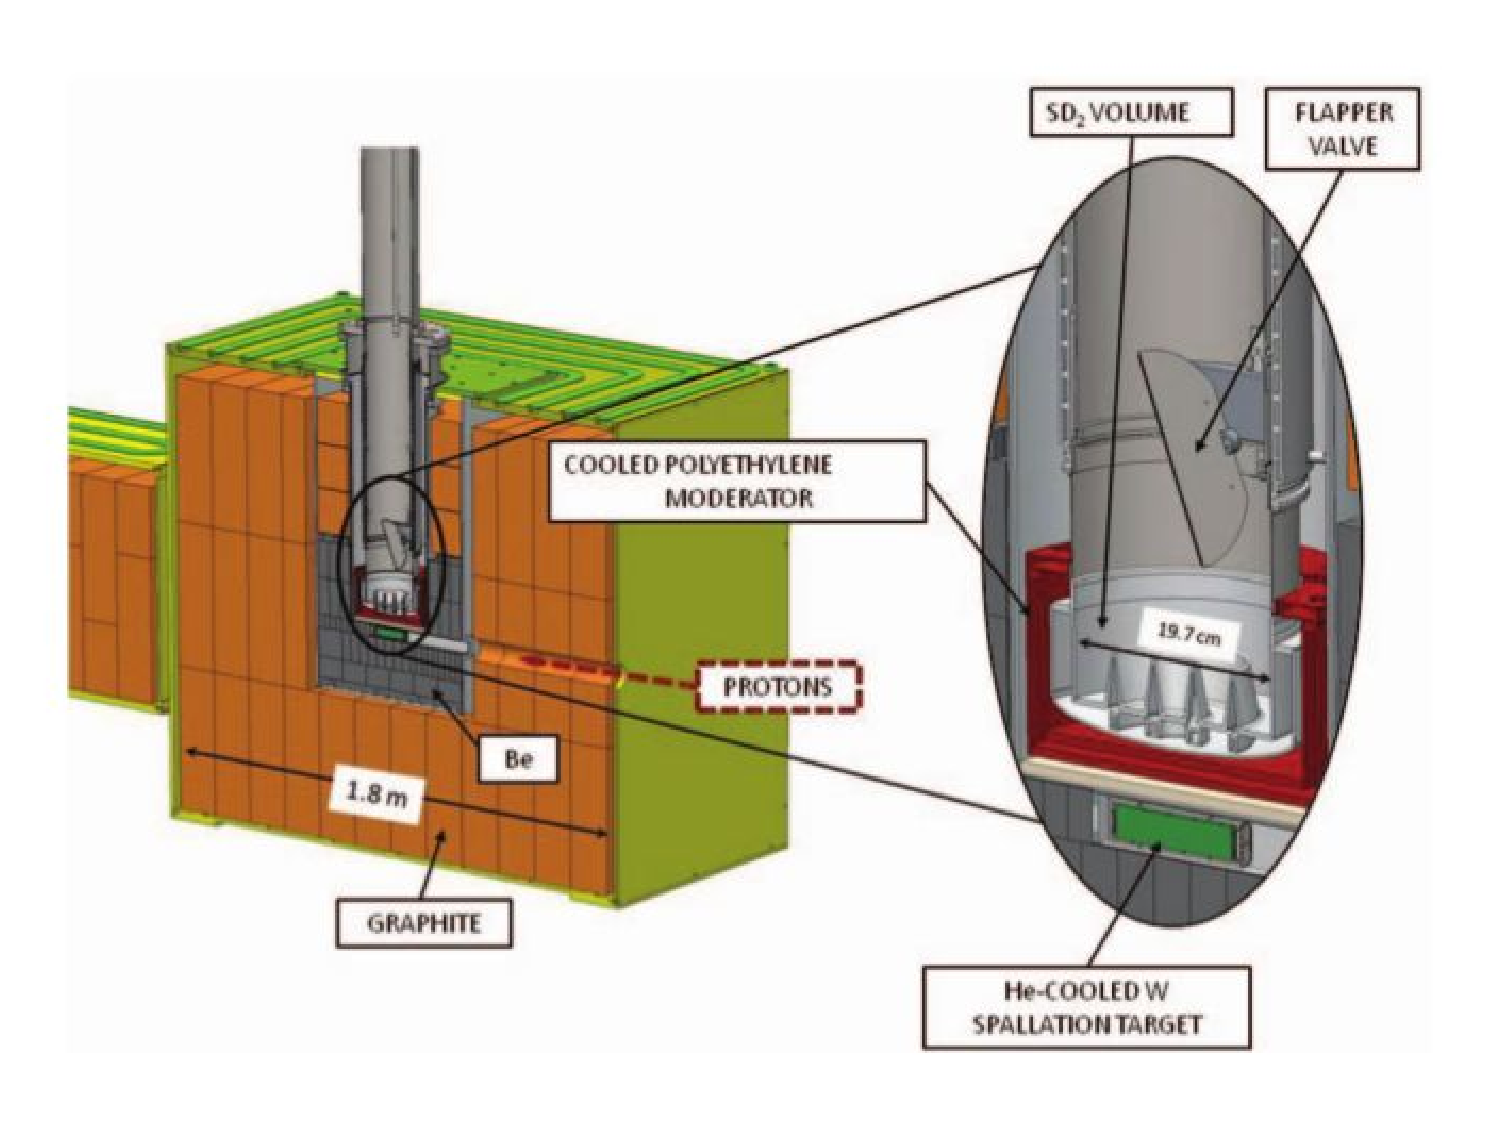
\includegraphics[scale=0.48]{2-UCNAExperiment/source_figure.pdf} 
  \caption{UCN source schematic. Inlay is a zoom in on the
    $\mathrm{SD}_2$ cell \cite{saunders2013performance}.}
  \label{fig:sourceFig}
\end{figure}

Detailed descriptions of the UCN source can be found in
\cite{saunders2004demonstration,morris2002measurements,saunders2013performance}, with
more recent improvements given in \cite{ito2017performance}. The state of the
UCN source today is different than what is described hereafter, with a substantial
increase in UCN production.

A schematic to assist in the understanding of the source at the time of data-taking
for this analysis is found in figure
\ref{fig:sourceFig}. The process begins with delivery of protons from the 800~MeV proton
accelerator operated in pulsed mode, with pulses repeated at a rate of 0.2~Hz.
The protons strike a helium-cooled tungsten target (12~cm long) and produce
spallation neutrons at roughly 20~MeV. The spallation target is surrounded by
a room temperature beryllium reflector to help direct as many neutrons as
possible towards the UCN source. The solid deuterium ($\mathrm{SD}_2$) UCN source
is located directly above the tungsten target, housed in a liquid helium
cooled cryostat. Prior to entering the $\mathrm{SD}_2$ source, neutrons
pass through a 1~cm thick moderator made of polyethylene beads cooled with the boil off gas
from the cooling of the $\mathrm{SD}_2$ source in the cryostat.
UCN are produced using the superthermal interaction of a cold neutron with the $\mathrm{SD}_2$,
which transfers most of the neutron's energy to a phonon in the crystal \cite{golub1991ultra}.

The $\mathrm{SD}_2$ source is a cylinder 19.7~cm in diameter and 5.7~cm tall. There
is a collection of ``fins'', or vertical teeth-like structures, located in
the bottom of the aluminum cryostat to increase the surface area of contact between the
$\mathrm{SD}_2$ and the liquid helium cooled surface. The surface of the cryostat
is coated with beryllium to reflect as many UCN as possible within the UCN source. Above
the $\mathrm{SD}_2$ is a flapper valve which opens to let UCN out of the source and
prevented UCN from re-entering the $\mathrm{SD}_2$ to reduce upscattering and loss of UCN.

Once a UCN passes the flapper, it is guided along a 1~m vertical guide coated with $^{58}\mathrm{Ni}$.
At this point, the UCN enter stainless steel horizontal guides for transportation from
the biological shielding that surrounds the source. The higher 342~neV potential of the
the $^{58}\mathrm{Ni}$ ensures that all neutrons which are capable of being guided by the
stainless steel (189 neV potential) are confined within the entirety of the vertical guide
\cite{saunders2013performance}. Upon looking at figure \ref{fig:guides}, one sees that
there are two $45\degree$ bends in the stainless steal guides to remove neutrons still
exceeding the UCN regime \cite{plaster2012}.

\begin{figure}[h]
  \centering
  \includegraphics[scale=0.48]{2-UCNAExperiment/experimentalSetup.png} 
  \caption{Schematic of guides and layout of the UCNA experiment \cite{plaster2012}.}
  \label{fig:guides}
\end{figure}

Once the UCN exit the shielding, they are guided along stainless steel guides
through a gate valve which allows for separation of the UCNA apparatus from the UCN
source while the proton beam is on, thus allowing for background measurements in
the spectrometer
during $\beta$-decay running conditions (proton beam operating, but void of UCN).
Beyond the gate valve is a 6~T pre-polarizing magnet (PPM). The purpose of the PPM
is to minimize the loss of UCN during transport through the Zr foil used to separate
the vacuum in the UCN source from the vacuum in the rest of the apparatus. The neutrons
are nominally polarized longitudinally after passing through the PPM's longitudinal field.

Beyond the PPM, the guides switch to electropolished copper (168 neV potential) to
maintain the initial polarization of the neutrons. Just downstream of the PPM
is the ``switcher'' valve. When the valve is open, the downstream guides are connected
to the guides coming from the PPM carrying UCN. Upon closing the switcher valve,
the downstream guides are redirected to a $^3\mathrm{He}$ 
UCN detector \cite{morris2009multi} used in polarimetry measurements.

Upon bypassing the switcher,
the UCN are guided through the 7~T primary polarizing magnet (or AFP magnet). At this point
the guides switch to 100~cm of diamondlike carbon coated quartz guides \cite{mammei2010thin}
for passage through the Adiabatic Fast Passage (AFP) spin flipper \cite{holley2012high}.
The guides then switch back to circular copper guides before coupling to a rectangular
(4~cm width $x$ 7~cm height) copper guide which transports the neutrons into the 1~T field
inside the Superconducting Spectrometer (SCS).

Prior to the beginning of running in 2011, a shutter was installed between the decay trap and
the guides used to close the decay trap off from the guides. During normal $\beta$-decay
runs, the shutter is open allowing neutrons to flow into (and out of) the decay trap as they are
created in the source. The shutter then closes at the beginning of a depolarization run, which immediately
follows every $\beta$-decay run, to allow for draining of the guides prior to a depolarization
measurement. This will be discussed in more detail later.

\section{Neutron Polarization} \label{sec:polarization}

The neutrons are initially polarized utilizing the $\boldsymbol{-\mu\cdot B} \approx \pm 60$~neV/T
potential. The UCN pass through the 6~T pre-polarizing magnet and then
through the 7~T primary AFP polarizing magnet. Neutrons with spin
aligned to the field (remember that the magnetic moment of the neutron is negative and so is antialigned
to the spin) see a positive (repulsive) potential of 420~neV from the 7~T magnet, and thus all
UCN in this spin state are reflected. The opposite spin state sees an attractive potential
and is transmitted, thus producing
a completely polarized population of UCN beyond the AFP magnet.
At this point, the neutrons pass through the AFP spin flipper. If the spin flipper is on, the spins
undergo a $\pi$ spin-flip before being loaded into the decay trap, and when off, the spins are
loaded in the same state that was selected by the AFP magnet.

A detailed description of the spin flipper can be found in \cite{holley2012high}. In short, the
flipper works under the premise of nuclear magnetic resonance (NMR) and utilizes a sinusoidally
varying magnetic field ($B_1$) that is transverse to the primary holding field ($B_0\approx 1$~T).
If there is a finite region where the $B_1$ field exists, i.e. it is zero outside this region and only
the $B_0$ holding field exists, it can be shown that as a spin passes through this region
it will undergo a $\pi$ spin-flip if at some point on the interval
the frequency $\omega$ of the rotating field $B_1$ is equal to the
Larmor precession frequency $\omega_{\mathrm{L}}$ of the spin about the holding field $B_0$.
To ensure that $\omega = \omega_L$ at some point
on the neutron's trajectory through this interval,
a gradient was introduced in the holding field $B_0$ while the frequency of
the rotating field was held constant. With proper tuning, the resonance condition is met, and as long
as adiabaticity is maintained, the spin flips direction. The conditions for adiabaticity defined in terms
of pertinent field parameters for this setup can be found in
\cite{holley2012high}. Testing of the apparatus indicates an efficiency of $0.9985\pm0.0004$ \cite{holley2012high}.

\begin{figure}[h]
  \centering
  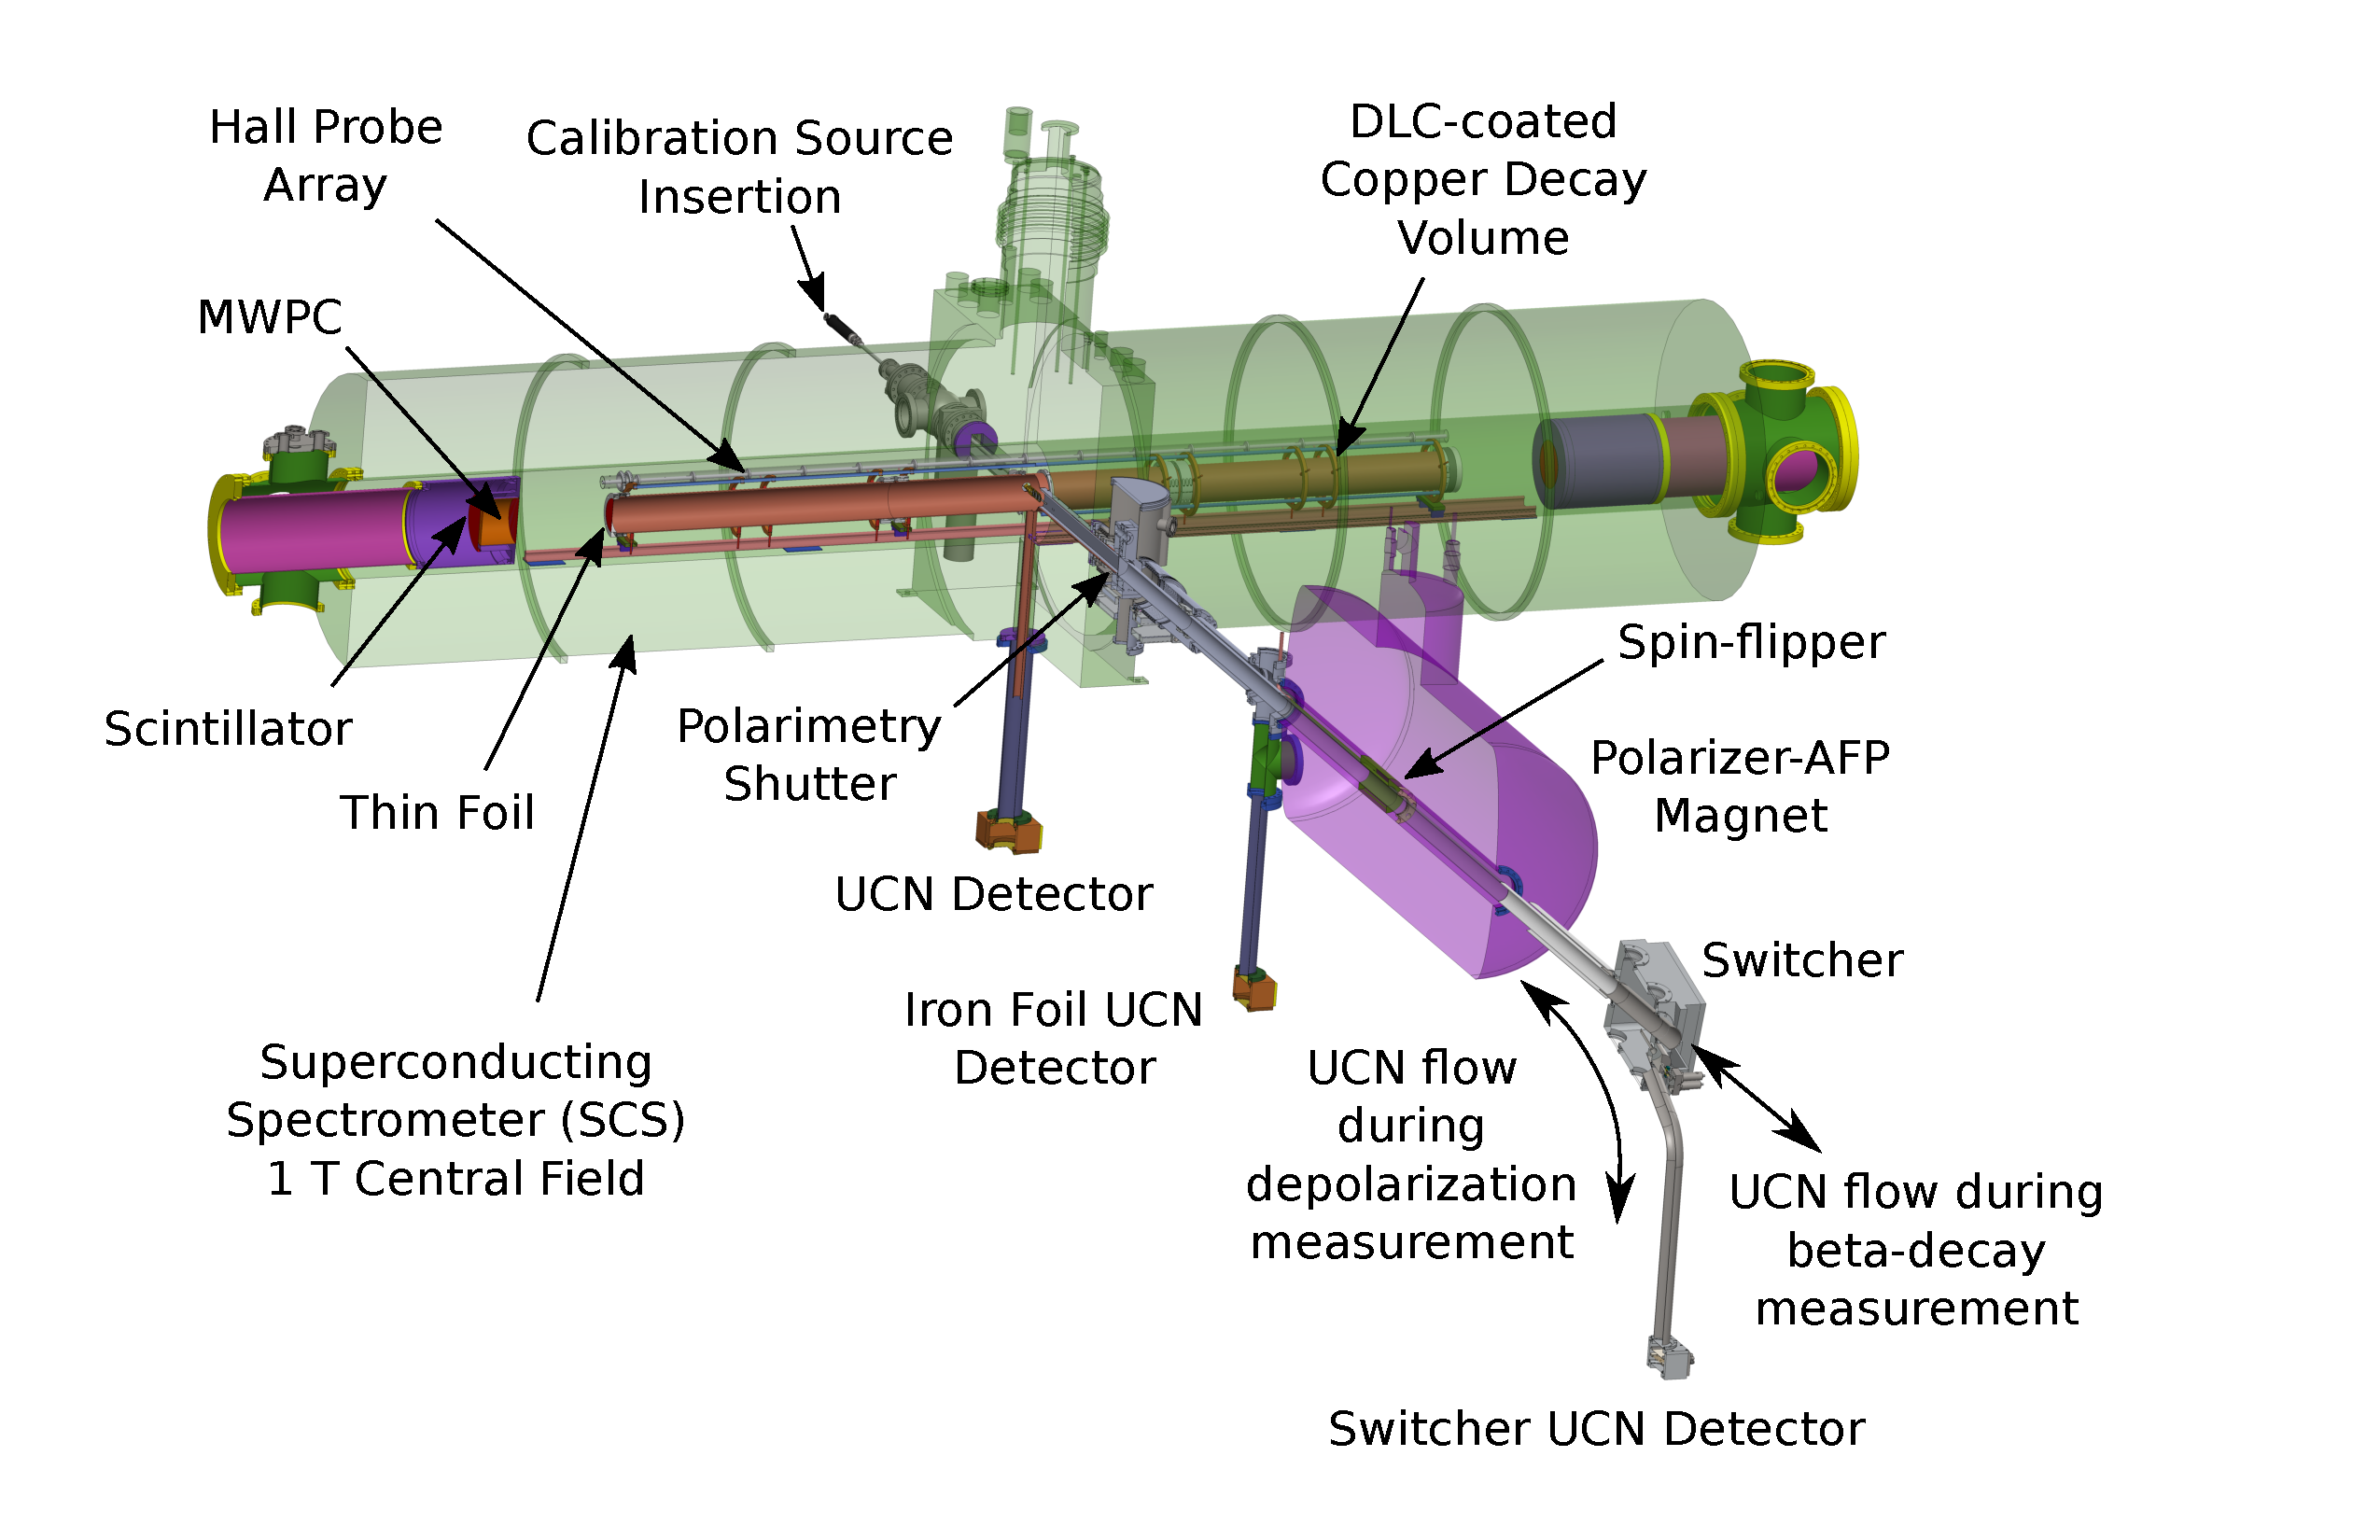
\includegraphics[scale=0.38]{2-UCNAExperiment/UCNAFig.pdf} 
  \caption{Detailed rendering of the experimental area. }
  \label{fig:setup}
\end{figure}

\section{Super-conducting Solenoidal Spectrometer}

The spectrometer consists mainly of the superconducting solenoidal magnet designed to produce
the 1~T central field, a decay trap to contain the UCN until they decay, and detector
packages located at each end of the spectrometer to detect decay electrons after they spiraled
about the field lines towards either detector. The detectors are referred to as
East and West based on their orientaion in the experimental area.
Brief descriptions of the main components follow.

\subsection{Decay Trap}
The decay trap is situated at the center of the spectrometer within the 1~T magnetic
field. The cylindrical 300 cm in length, 12.4 cm in width decay trap is made of electropolished Cu
to confine as many UCN as possible. Typically the vacuum within the decay trap and the guides
upstream to the Zr foil which separated the source vacuum from the experimental apparatus was about
$10^{-5}$~Torr. The density of UCN in the decay trap was monitored using a $^3\mathrm{He}$ UCN detector
directly below a 0.64~cm hole in the decay trap.

One of the main differences between the 2011-2012 and 2012-2013 run periods was the thickness and
material of the decay trap endcaps. In both geometries the endcaps were coated with 150~nm of
Be (potential 252 neV) to aid in reflecting neutrons to confine them. The 2011-2012 endcaps
were 500~nm Mylar on both the East and West detectors, while the 2012-2013 endcaps were made of 6F6F
\cite{hoedl2003} and were 130~nm (East) and 180~nm (West) thick. The change in endcap thickness
is the primary reason for analyzing the two sets of data separately, as this changes the
systematics involving electron backscattering. 

\subsection{Magnetic Field} \label{ssec:MagneticField}

The general requirements for the magnetic field within the decay trap was that it must be aligned with
the axis of the decay trap to define the axis of polarization, strong enough to confine the larmor
radius of the decay electrons as they spiral toward the detectors, and uniform enough that
electrons will not be reflected.

The necessity for a uniform magnetic field follows from consideration of the flux contained
within the spiral of the electron around the magnetic field lines. From \cite{jackson1999}
we know the flux, $Br_e^2$, is an adiabatic invariant, which means so is $p_\perp^2/B$ where
$p_\perp$ is the transverse momentum of the spiraling electron and $p = \sqrt{p_\perp^2+p_\parallel^2}$.
Given this, there exists a condition for reflection when an electron originates in a field $B_0$
with initial momentum $p_0 = \sqrt{p_{0,\perp}^2+p_{0,\parallel}^2}$
and encounters a field $B_{\mathrm{max}}$,
%
\begin{equation}
  \frac{B_{\mathrm{max}}-B_0}{B_0} > \frac{p^2_{0,\parallel}}{p^2_{0,\perp}}.
  \label{eq:fieldReflection}
\end{equation}
%
A field uniformity of $10^{-4}$ was determined sufficient to remove appreciable effect
on the asymmetry \cite{plaster2008solenoidal}.

The magnet, constructed by American Magnetics, Inc., is a warm-bore 35~cm diameter, 4.5~m
long superconducting solenoid (SCS magnet). Technical details of the magnet can be found in
\cite{plaster2008solenoidal, plaster2012}. An important aspect of the magnetic field not mentioned
previously is the field expansion from 1~T to 0.6~T beyond the decay trap windows but prior to
the wirechambers. This field expansion decreases the pitch angle of the electron,
defined as
$\theta = \arccos(p_{\parallel}/p)$, as it
enters the detector package as seen from the earlier stated adiabatic invariant $p_\perp^2/B$
coupled with conservation of momentum. Decreasing the pitch angle decreases the probability
of backscattering substantially.

\begin{figure}[h]
  \centering
  
\includegraphics[scale=0.38]{2-UCNAExperiment/ImageHolder.pdf} 
  \caption{Typical field profile from 2011-2012 run period.}
  \label{fig:field_profile}
\end{figure}

In 2011-2012 and 2012-2013, the magnetic field was not as uniform as reported in 
\cite{plaster2008solenoidal} due to damage to the shim coil persistence heater switches
due to multiple magnet quenches \cite{plaster2012}. A typical field profile can be seen
in figure \ref{fig:field_profile}, where the uniformity is at the $10^{-3}$ level, but there is
pronounced dip in the center. Electrons
that originate in the dip region can become trapped if the condition in equation
\ref{eq:fieldReflection} is satisfied. The electron then only exits the field dip
upon scattering from the residual gas in the decay trap which randomized the direction
of the electron. The effect
on the asymmetry from the field
dip is addressed as a systematic
uncertainty in section \ref{sssec:MagFieldSyst}.


\subsection{Detector Packages}

\begin{figure}[h]
  \centering
  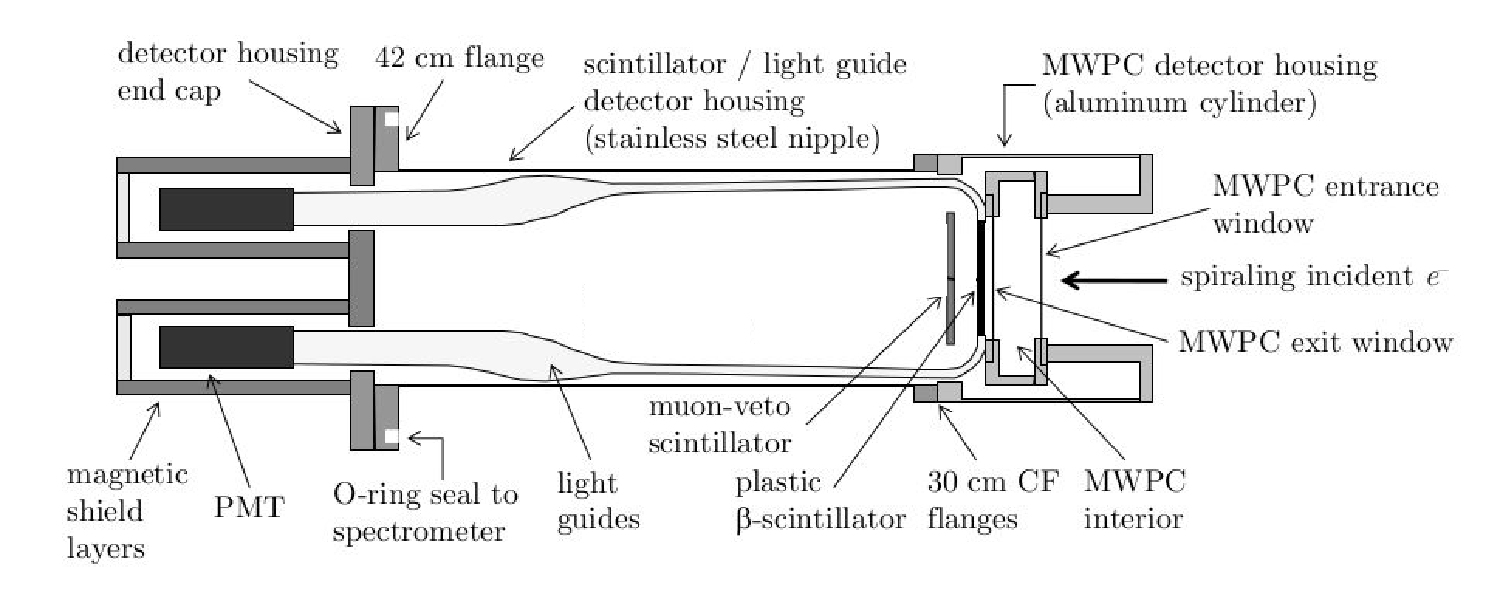
\includegraphics[scale=0.6]{2-UCNAExperiment/detector_setup.pdf} 
  \caption{Schematic of the detector packages \cite{plaster2012}.}
  \label{fig:detectors}
\end{figure}

\subsubsection{Multiwire Proportional Chamber} \label{sec:ExpMWPC}

The multiwire proportional chamber (MWPC, or sometimes simply called the wirechamber)
\cite{ito2007,plaster2012} is
utilized to reconstruct the position of the electron events and to reduce the ambient
backgrounds. The MWPC consists of an anode plane in between two cathode planes, with the cathode
planes oriented perpendicular to one another to allow for position reconstruction in both directions
transverse to the axis of the SCS. There are
64 wires in each plane with 2.54~mm spacing between each wire. The spatial extent of the
MWPC is $16.3 \times 16.3\mathrm{ cm}^2$ which maps to
$\sqrt(0.6) (\times 16.3 \times 16.3\mathrm{ cm}^2) = 12.6 \times 12.6\mathrm{ cm}^2$ coverage
within the decay trap (remember the decay trap is within the 1~T field while the detectors
are in the field expansion region with field of 0.6~T), thus the wirechamber covers the full
decay trap exit. The anode wires are $10\mathrm{ \mu{n}}$ in diameter while the cathode
wires are $78.2\mathrm{ \mu{n}}$ in diameter, with the diameter of the cathode wires slightly
larger than in previous run periods ($50\mathrm{ \mu{n}}$).

Charged particles passing the MWPC ionize the gas, and the \~2700~V bias between the anode and
cathode plains causes the ions and electrons to drift and induce a signal in the wires (ADD TO THIS).
The anode wires are read out as a summed signal, with all 64 wire signals summed corresponding to
a single ADC channel. This signal is typically used in relating the total signal in the MWPC
to an energy deposited within the wirechamber. The cathode wires are read out in groups of four
consecutive wires, so there are 16 ADC channels for each wirechamber cathode plane. These 16
``wires'' (as we will call them from now on) are used for position reconstruction. Either
signal can be effectively used for the MWPC software trigger.

The fill
gas chosen for the MWPC should be low Z ( low atomic number) to minimize the backscattering from heavy nuclei,
but also electron dense to increase the ionization efficiency. Thus complex large molecules
made up of low Z nuclei are good candidates.
The MWPC was primarily filled with neopentane ($\mathrm{C}_5\mathrm{H}_{12}$) gas at a pressure of
100~Torr, chosen to ensure enough gain for electrons within the $\beta$-decay spectrum. For a
short time period in 2012-2013, the neopentane ran out and isobutane ($\mathrm{C}_5\mathrm{H}_{10}$)
was used instead. Separate simulations were used for the isobutane runs, but no appreciable
difference was noticed.

The windows on the wirechamber were made as thin as possible so as to reduce backscattering, but still
retain their integrity under the 100~T pressure difference between the SCS and the wirechamber. Events that
scatter off of the entrance window are particularly troublesome as they become missed backscattering events.
The chosen front window material was $6\mathrm{ \mu{n}}$ of aluminized Mylar reinforced with Kevlar strings
placed at 5~mm increments, and the exit window was also $6\mathrm{ \mu{n}}$ of aluminized Mylar \cite{mpmThesis}. 

The importance of the MWPC should not be understated. First of all, the position reconstruction allows for the
definition of a fiducial volume within the decay trap so that we can cut out events which may have interacted
with the decay trap walls. Such interactions change the energy/direction of the electron, so simply cutting them
out reduces the systematic correction necessary. Secondly, the scintillator's energy response is position
dependent, so the position of each event is needed to properly assign a reconstructed initial energy to
each electron event. The MWPC is also vital in identifying backscattering events by looking at the energy
deposited within the wirechamber, i.e. an event that backscatters off of the dead layer of the scintillator
will deposit energy in the MWPC above some software cut and can be identified. And last of all,
the wirechamber is highly insensitive to gamma rays, so by including a coincidence trigger between the wirechamber
and the scintillator the majority of the gamma background is removed.

\subsubsection{Scintillator}

A 15~cm diameter, 3.5~mm thick plastic scintillator \cite{plaster2012}
from Eljen Technology (EJ-204) was located beyond the
MWPC. The maximum stopping distance for an endpoint (782~keV) electron is 3.1~mm, so the
scintillator is capable of reconstructing the entire energy spectrum. To transport the
scintillation light out of the 0.6~T field to the photomultuplier tubes (PMT),
located \~1~m in a \~0.03~T field,
twelve light guides were coupled to the edge of the scintillator using optical grease.
From there, the twelve guides are adiabatically merged into four
larger guides which are attached to four Hamamatsu R7725 PMTs with custom bases \cite{hickerson2013}.
The light guides are merged and coupled to the PMTs in such a way that each PMT effectively
covers one quadrant of the scintillator, as will become clear when discussing the calibrations.
A hardware two-fold trigger, or two PMTs above discriminator threshold, is required for an
global trigger to be issued from the PMTs.

\subsubsection{Energy Calibration}

The scintillator energy calibration utilized the conversion electron lines from
(with dominant K-shell energies listed) $^{137}\mathrm{Ce}$
(130.3 keV), $^{113}\mathrm{Sn}$ (363.8 keV), and $^{207}\mathrm{Bi}$ (481.7~keV and 975.7 keV)
sources. These sources were placed on a source paddle and inserted into the side of the
decay trap while under vacuum, and then they were translated across the horizontal axis of the decay
trap. This method probed the position dependence of the scintillator, but only along one axis and
at discrete points. The full position response was captured using another method as will be
described later. Also detailed later in section \ref{sec:biGain}, the gain of the PMTs was monitored
and drifts corrected 
on a run-by-run basis using a $^{207}\mathrm{Bi}$ ``pulser'' system \cite{morris1976stable}.

\subsubsection{Muon Veto System}

Cosmic ray muons can create a scintillator two-fold trigger and pass the software trigger in
the MWPC, which means according to trigger logic they look like an electron. By identifying
the muons through means other than the scintillator or wirechamber. The first mechanism
is an argon/ethane sealed drift tube system \cite{rios2011sealed}. The drift tube veto sits
above the spectrometer, partially wrapped around the sides. Muons ionize the gas inside the
tube, and thus by checking for a coincidence in the drift tube, one can remove muons
and events from secondary electrons created by the muons. The second method of monitoring
the muon contamination is the use of scintillators placed directly behind the primary
electron scintillator as seen in figure \ref{fig:detector}. The primary detector
stops all $\beta$-decay electrons, so a coincident signal in the ``backing veto''
indicates that a muon or some other event passed through the detector package.

\section{Data Signals and Trigger Logic}

Details regarding the data acquisition system can be found in \cite{plaster2012,mpmThesis}, and
so the electronics will be left out of this discussion. Instead, what is more important for
understanding the work contained within this dissertation is the primary logic used to
determine an electron event, and the terminology used when discussing different signals.

The two primary types of signals we will use are ADC and TDC signals.
An ADC signal is a number related to a voltage output by a detector component, and this
signal may either be an integrated signal or a peak sensing signal. Either way, it is related
to the ``strength'' of the signal as seen by the detector component, or the energy deposited
in most cases. An example of an ADC signal can be seen in figure \ref{fig:ADCsig}, where we show the
detector output over one run for a single PMT during a $\beta$-decay run.
The second signal used is a TDC signal, which for our purposes is
just a timing signal to indicate when a detector component triggered, or if it triggered at all.
An example TDC signal can be
seen in figure \ref{TDCsig}.

\begin{figure}
  \centering
  \subfloat[Raw ADC signal]{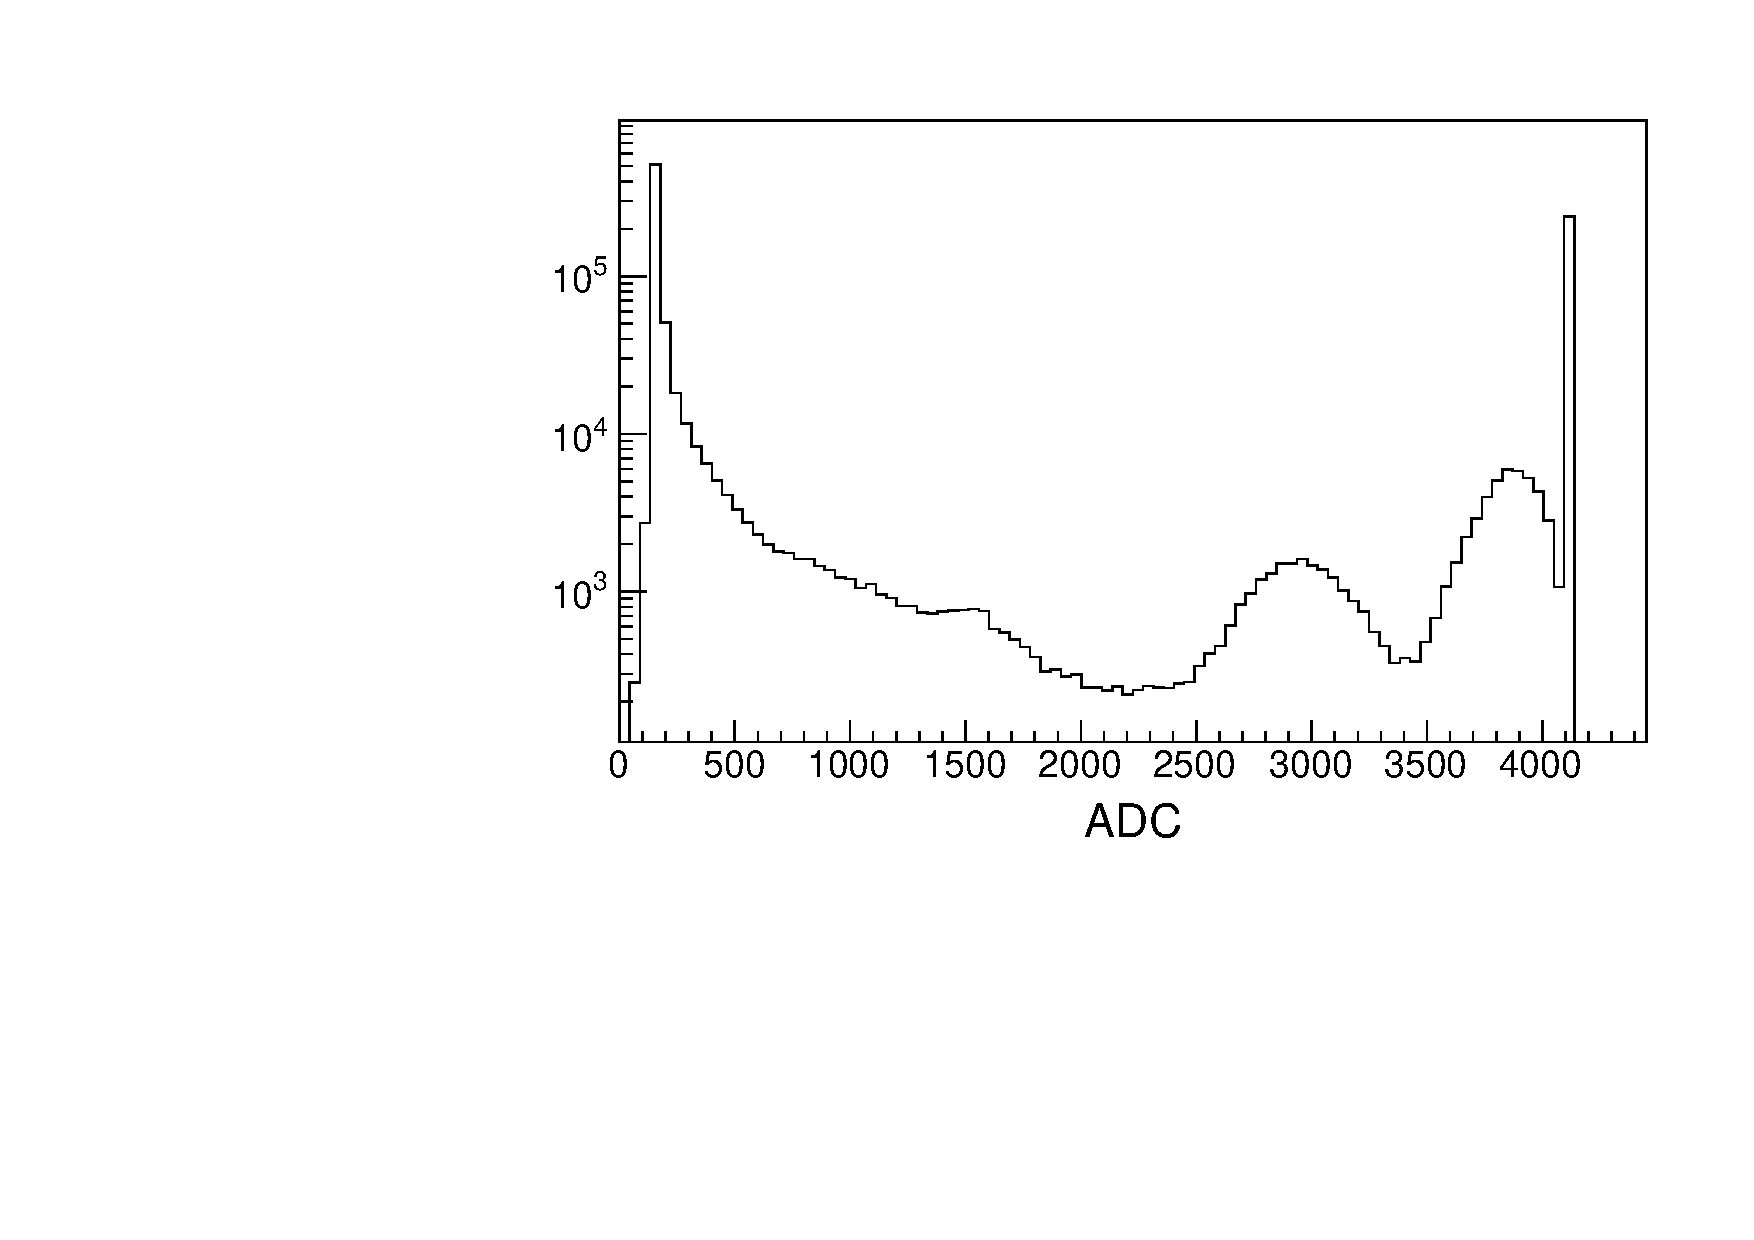
\includegraphics[page=1,scale=0.38]{2-UCNAExperiment/rawADCsignal17126.pdf}}
  \subfloat[Raw ADC signal with two-fold scintillator trigger applied]{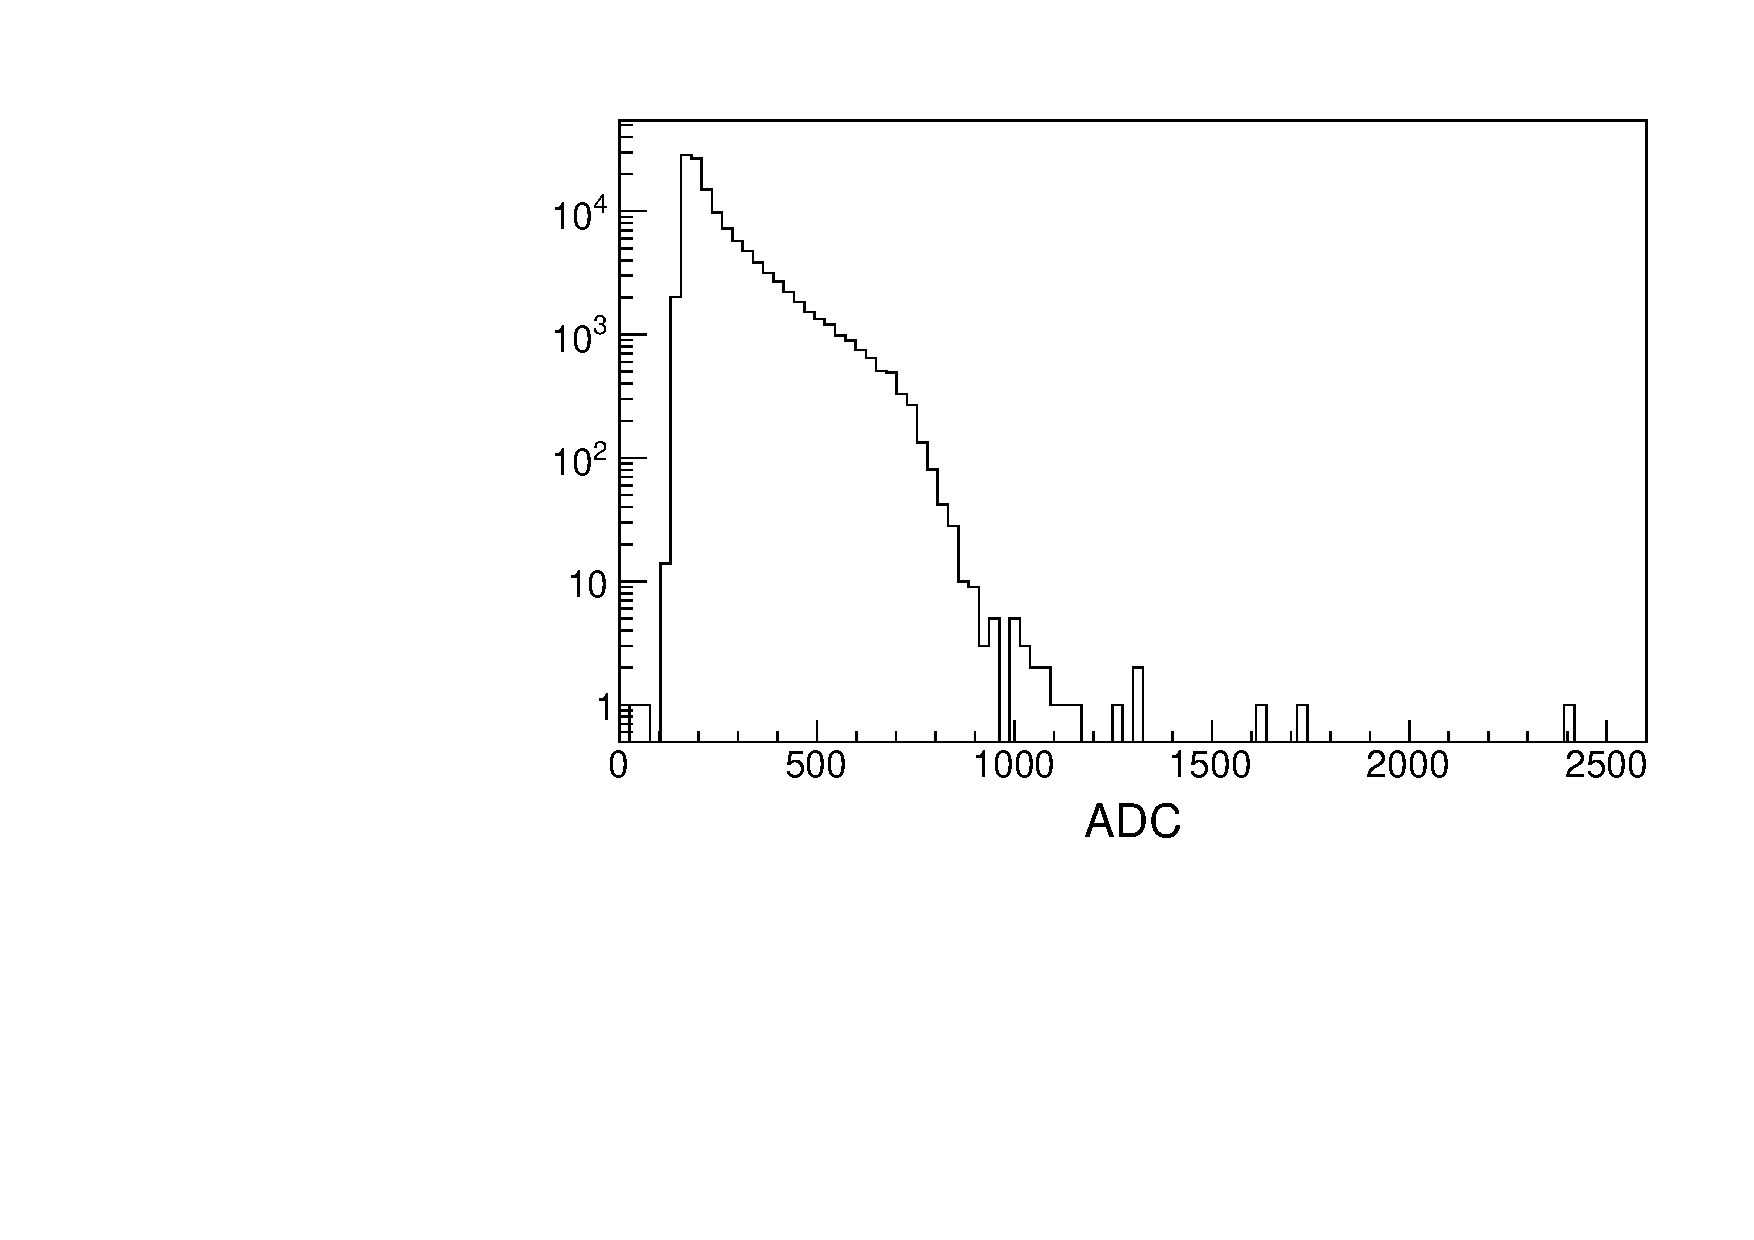
\includegraphics[page=1,scale=0.38]{2-UCNAExperiment/rawADCsignal17126_betaEast.pdf}}
  \caption{Comparison of the raw ADC signal from a single PMT for any global trigger a.) and upon requiring a two-fold PMT trigger
    on the side of the PMT of interest b.). This type of cut is part of the electron trigger along with a coincidence with the wirechamber.}
  \label{fig:ADCsig}
\end{figure}

\begin{figure}
  \centering
  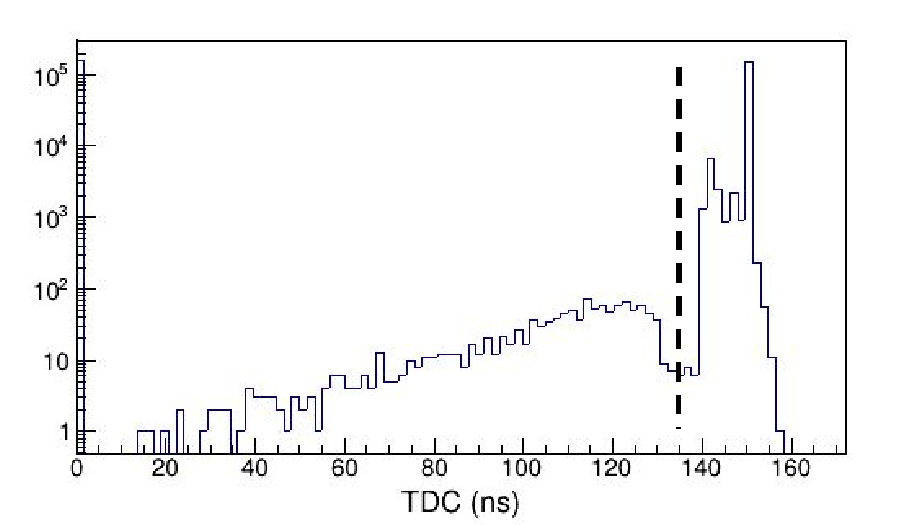
\includegraphics[page=1,scale=0.60]{2-UCNAExperiment/TDCSignal.pdf}
  \caption{Example TDC signal (converted to nanoseconds) from a $\beta$-decay run.
    Note that the horizontal axis is technically time since trigger, so a longer time indicates an earlier
    trigger.The dashed line
    indicates the cut used to separate a self-trigger (right of the dashed line) from a backscattering trigger
    (left of the dashed line).  The events at $t=0$ are events which did not create a self-trigger.}
  \label{fig:TDCsig}
\end{figure}


Several types of signals can generate a global trigger, where the data acquisition system (DAQ)
reads all possible inputs. These include:
%
\begin{itemize}
\item UCN monitor $-$ used to monitor the UCN production at various
  stages along the experimental apparatus
\item $^{207}\mathrm{Bi}$ pulser event $-$ This is a high threshold, single PMT trigger, so if one PMT
  has a trigger above a preset high threshold, but no other PMT has any trigger, this indicates the
  pulser created the trigger at the PMT and not the scintillator. This will be addressed more in the
  next chapter.
\item LED pulser $-$ An LED system was in place to assist in correcting any non-linearity in the
  PMT response. This was not utilized in this analysis.
\item Two-fold PMT trigger $-$ two of the four PMTs on one side must have signal above a pre-set
  threshold. This two-fold trigger indicates a particle deposited energy in the scintillator,
  distinguishing it from noise in a single PMT, a $^{207}\mathrm{Bi}$ pulser event, or an LED event.
\end{itemize}


%UCN monitor detectors with a signal over threshold,
%a single PMT high energy trigger which indicates a $^{207}\mathrm{Bi}$ gain monitor trigger,
%or a two-fold PMT trigger.

The two-fold PMT trigger is of most importance for us, as this indicates
that there was sufficient energy deposition in the scintillator to be an electron event.
The hardware trigger does not
discriminate between what type of event may have created the trigger though, so any particle
that can deposit energy in the scintillator could have been the culprit. For this, we rely
on methods already highlighted in above sections. By applying a software trigger to
the wirechamber, we can require that any event which created a two-fold scintillator trigger
in detector 1 must also pass the software trigger in MWPC 1. This essentially removes the
gamma background, as the wirechamber is virtually transparent to a gamma.
Then by checking for muon veto signals above some software threshold we eliminate
cosmic ray muon backgrounds, leaving us with almost all electron events. Of course there are
some background events that always make it into the analysis, but these are also accounted for
as will be discussed.

Along with ADC signals proportional to energy deposition, all PMTs also report hardware trigger
timing information (TDC signal). For backscattering events which trigger both detectors, we use the timing
to determine the primary side, or the initial direction of the electron. This can be seen in
figure \ref{TDCsig}. The dashed line indicates the position of a cut to separate a primary trigger
from a backscattering trigger. An acceptable event either has a single primary trigger or a primary
trigger on one side and a backscattering trigger on the other side. 



%%%%%%%%%%%%%%%%%%%%%%%%%%%%%%%%%%%%%%%%%%%%%%%%%%%%%%%%%%%%%%%%%%%%%%%%%%%%%%


\section{Data Taking Structure}

The data is broken into three types of run periods, namely $\beta$-decay data, source calibration, and
Xe position mappping. The latter two determine the parameters of the energy calibration to be
applied to the data runs. The source calibration and Xe position mapping run periods
occur periodically throughout each data set and are applied to surrounding $\beta$-decay runs. This
creates different subsets of data to which each calibration is applied, as will be illustrated
throughout the rest of this dissertation. Here we simply highlight the structure of the
$\beta$-decay runs, and one should take note that the source calibrations and Xe position map periods
are spaced throughout.

\subsection{$\beta$-decay run structure}
We utilize what we call an octet run structure, where each octet contains a total of twenty-four
runs, eight of which are $\beta$-decay data runs, eight of which are background runs, and eight
of which are depolarization runs. The octet is further split into two halves, A and B, which define
the order of the runs within them as seen in table \ref{tab:octetStructure}. Whether the A structure
or the B structure comes first within an octet is determined randomly. There are four $\beta$-decay
runs of each spin-state (aligned and anti-aligned to the magnetic field in the spectrometer), and their
accompanying background runs allow for background subtraction. 

\begin{table}[h]
  \caption{Octet structure, where $\pm$ indicates spin flipper on/off,
    B refers to background run, D refers to depolarization run, and $\beta$
    refers to $\beta$-decay runs.} 
  \centering
  \begin{tabular}{llllllllllll}
    \hline \hline \\ [-1.75ex]
    A1 & A2 & A3 & A4 & A5 & A6 & A7 & A8 & A9 & A10 & A11 & A12 \\ 
    B$^-$ & $\beta^-$ & D$^-$ & B$^+$ & $\beta^+$ & D$^+$ & $\beta^+$ & D$^+$ & B$^+$ & $\beta^-$ & D$^-$ & B$^-$ \\
    \hline \\ [-1.75ex]
    B1 & B2 & B3 & B4 & B5 & B6 & B7 & B8 & B9 & B10 & B11 & B12 \\
    B$^+$ & $\beta^+$ & D$^+$ & B$^-$ & $\beta^-$ & D$^-$ & $\beta^-$ & D$^-$ & B$^-$ & $\beta^+$ & D$^+$ & B$^+$ \\
    \hline
  \end{tabular}
  \label{tab:octetStructure}
\end{table}



\section{Backscattering} \label{sec:backscattering}
Before moving forward, it is important to formally introduce the different
backscattering events, as they will be referenced often. A backscattering
event is an electron event initially emitted towards one detector, but that
is scattered through a large enough angle that its momentum is reversed and
it travels to the opposite detector. Some of these events are backscattered
by a detector component and can therefore be identified as having backscattered
due to energy deposition on both sides,
while others backscatter without depositing enough energy (or backscatter prior
to reaching the detector) and therefore become what we call ``missed''
backscattering events. Missed backscattering events are problematic as they
are assigned the wrong intitial direction and therefore systematically effect
the asymmetry.

\begin{figure}[h]
\centering
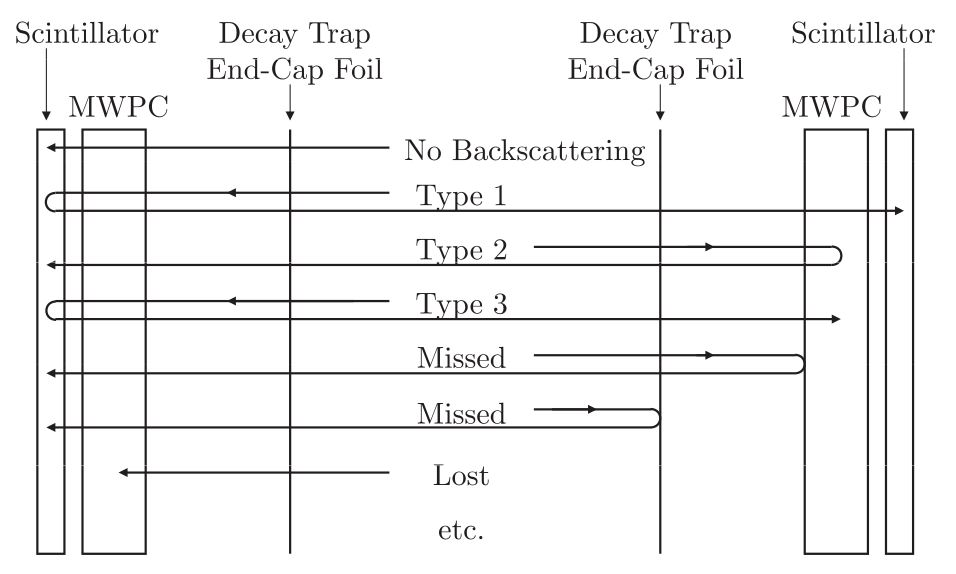
\includegraphics[scale=.4]{3-UCNAAnalysis/backscatterSchematic.png}
\caption{Schematic of different event types and the trigger logic involved with identifying
  each type \cite{plaster2012}.}
\label{fig:backscatterSchematic}
\end{figure}

Based on which detector components trigger, we classify events
into those that do not backscatter
(Type 0) and those that do backscatter (Types 1, 2, and 3) \cite{plaster2012}.
A schematic of the different event types can be seen in figure \ref{backscatterSchematic}.
Type 0 events
trigger one scintillator and one MWPC on the same side, while Type 1 events trigger
both scintillators and both MWPCs. For such events, we assign the initial
direction to the triggering detector for Type 0 and to the earlier triggering detector
for Type 1. Type 2/3 events comprise a class of events that backscatter and trigger both
MWPCs, but only trigger a single scintillator.
The initial direction of such events can
not be determined from trigger logic alone, as can be demonstrated by considering two events
which look identical under trigger logic.
For example, let ``Event 1'' denote an event that initially backscatters off
of MWPC 1 before reaching scintillator 1
and then traverses the length of the decay
trap to trigger both MWPC 2 and scintillator 2 on the opposite side.
Then, suppose ``Event 2'' denotes another event emitted
in the opposite direction to event 1. Suppose this event
triggers MWPC 2 and scintillator 2
only to backscatter from the scintillator and travel to MWPC 1 and stop short
of scintillator 1. Both events trigger MWPC 1 and 2 and scintillator 2,
but the two events had opposite initial directions, so inclusion of the
two events without further knowledge of their initial direction creates
a dilution to the asymmetry.

An important distinction, however, does exist between Type 2 and Type 3 events:
Type 2 events only pass through the MWPC on the
triggering scintillator side once, whereas Type 3 events scatter from
the scintillator, and therefore pass through the MWPC twice on
the triggering side. We can consequently apply a cut on the energy deposited in
the MWPC on the triggering side to statistically assign
Type 2/3 events to the correct side.
This drastically reduces
Monte Carlo corrections for such backscattering events as simulation indicates we
properly identify $>80\%$ of all Type 2/3 events across all energies using this
technique, a marked
improvement over the roughly $50\%$ misidentification rate without separation.








